% Options for packages loaded elsewhere
% Options for packages loaded elsewhere
\PassOptionsToPackage{unicode}{hyperref}
\PassOptionsToPackage{hyphens}{url}
\PassOptionsToPackage{dvipsnames,svgnames,x11names}{xcolor}
%
\documentclass[
  12pt,
  letterpaper,
]{article}
\usepackage{xcolor}
\usepackage[margin=1in]{geometry}
\usepackage{amsmath,amssymb}
\setcounter{secnumdepth}{-\maxdimen} % remove section numbering
\usepackage{iftex}
\ifPDFTeX
  \usepackage[T1]{fontenc}
  \usepackage[utf8]{inputenc}
  \usepackage{textcomp} % provide euro and other symbols
\else % if luatex or xetex
  \usepackage{unicode-math} % this also loads fontspec
  \defaultfontfeatures{Scale=MatchLowercase}
  \defaultfontfeatures[\rmfamily]{Ligatures=TeX,Scale=1}
\fi
\usepackage{lmodern}
\ifPDFTeX\else
  % xetex/luatex font selection
\fi
% Use upquote if available, for straight quotes in verbatim environments
\IfFileExists{upquote.sty}{\usepackage{upquote}}{}
\IfFileExists{microtype.sty}{% use microtype if available
  \usepackage[]{microtype}
  \UseMicrotypeSet[protrusion]{basicmath} % disable protrusion for tt fonts
}{}
\makeatletter
\@ifundefined{KOMAClassName}{% if non-KOMA class
  \IfFileExists{parskip.sty}{%
    \usepackage{parskip}
  }{% else
    \setlength{\parindent}{0pt}
    \setlength{\parskip}{6pt plus 2pt minus 1pt}}
}{% if KOMA class
  \KOMAoptions{parskip=half}}
\makeatother
% Make \paragraph and \subparagraph free-standing
\makeatletter
\ifx\paragraph\undefined\else
  \let\oldparagraph\paragraph
  \renewcommand{\paragraph}{
    \@ifstar
      \xxxParagraphStar
      \xxxParagraphNoStar
  }
  \newcommand{\xxxParagraphStar}[1]{\oldparagraph*{#1}\mbox{}}
  \newcommand{\xxxParagraphNoStar}[1]{\oldparagraph{#1}\mbox{}}
\fi
\ifx\subparagraph\undefined\else
  \let\oldsubparagraph\subparagraph
  \renewcommand{\subparagraph}{
    \@ifstar
      \xxxSubParagraphStar
      \xxxSubParagraphNoStar
  }
  \newcommand{\xxxSubParagraphStar}[1]{\oldsubparagraph*{#1}\mbox{}}
  \newcommand{\xxxSubParagraphNoStar}[1]{\oldsubparagraph{#1}\mbox{}}
\fi
\makeatother


\usepackage{longtable,booktabs,array}
\newcounter{none} % for unnumbered tables
\usepackage{calc} % for calculating minipage widths
% Correct order of tables after \paragraph or \subparagraph
\usepackage{etoolbox}
\makeatletter
\patchcmd\longtable{\par}{\if@noskipsec\mbox{}\fi\par}{}{}
\makeatother
% Allow footnotes in longtable head/foot
\IfFileExists{footnotehyper.sty}{\usepackage{footnotehyper}}{\usepackage{footnote}}
\makesavenoteenv{longtable}
\usepackage{graphicx}
\makeatletter
\newsavebox\pandoc@box
\newcommand*\pandocbounded[1]{% scales image to fit in text height/width
  \sbox\pandoc@box{#1}%
  \Gscale@div\@tempa{\textheight}{\dimexpr\ht\pandoc@box+\dp\pandoc@box\relax}%
  \Gscale@div\@tempb{\linewidth}{\wd\pandoc@box}%
  \ifdim\@tempb\p@<\@tempa\p@\let\@tempa\@tempb\fi% select the smaller of both
  \ifdim\@tempa\p@<\p@\scalebox{\@tempa}{\usebox\pandoc@box}%
  \else\usebox{\pandoc@box}%
  \fi%
}
% Set default figure placement to htbp
\def\fps@figure{htbp}
\makeatother





\setlength{\emergencystretch}{3em} % prevent overfull lines

\providecommand{\tightlist}{%
  \setlength{\itemsep}{0pt}\setlength{\parskip}{0pt}}



 


% Standard math packages
\usepackage{amsmath}
\usepackage{amsfonts}
\usepackage{amssymb}
\usepackage{bm}
\usepackage{amsthm}

% Custom shortcuts for number sets
\newcommand{\N}{\mathbb{N}}
\newcommand{\Z}{\mathbb{Z}}
\newcommand{\Q}{\mathbb{Q}}
\newcommand{\R}{\mathbb{R}}

% Theorem configurations
\theoremstyle{plain}
\newtheorem{theorem}{Theorem}
\newtheorem{proposition}{Proposition}
\theoremstyle{definition}
\newtheorem{definition}{Definition}

% Diagram and layout packages
\usepackage{tikz}
\usepackage{xcolor}
\usepackage{subcaption}
\usepackage{float}
\usepackage{enumitem}
\makeatletter
\@ifpackageloaded{caption}{}{\usepackage{caption}}
\AtBeginDocument{%
\ifdefined\contentsname
  \renewcommand*\contentsname{Table of contents}
\else
  \newcommand\contentsname{Table of contents}
\fi
\ifdefined\listfigurename
  \renewcommand*\listfigurename{List of Figures}
\else
  \newcommand\listfigurename{List of Figures}
\fi
\ifdefined\listtablename
  \renewcommand*\listtablename{List of Tables}
\else
  \newcommand\listtablename{List of Tables}
\fi
\ifdefined\figurename
  \renewcommand*\figurename{Figure}
\else
  \newcommand\figurename{Figure}
\fi
\ifdefined\tablename
  \renewcommand*\tablename{Table}
\else
  \newcommand\tablename{Table}
\fi
}
\@ifpackageloaded{float}{}{\usepackage{float}}
\floatstyle{ruled}
\@ifundefined{c@chapter}{\newfloat{codelisting}{h}{lop}}{\newfloat{codelisting}{h}{lop}[chapter]}
\floatname{codelisting}{Listing}
\newcommand*\listoflistings{\listof{codelisting}{List of Listings}}
\makeatother
\makeatletter
\makeatother
\makeatletter
\@ifpackageloaded{caption}{}{\usepackage{caption}}
\@ifpackageloaded{subcaption}{}{\usepackage{subcaption}}
\makeatother
\usepackage{bookmark}
\IfFileExists{xurl.sty}{\usepackage{xurl}}{} % add URL line breaks if available
\urlstyle{same}
\hypersetup{
  pdftitle={Nodes and Connections in a Complete Graph},
  colorlinks=true,
  linkcolor={blue},
  filecolor={Maroon},
  citecolor={Blue},
  urlcolor={Blue},
  pdfcreator={LaTeX via pandoc}}


\title{Nodes and Connections in a Complete Graph}
\author{}
\date{}
\begin{document}
\maketitle


While the basic formula for connections in a complete graph is a staple
of discrete mathematics, its behaviour reveals deep complexities when
viewed through a wider lens. This essay explores the dynamics of network
accumulation, the inversion of its quadratic growth, the vanishing
nature of its relative error, and an interesting geometric phenomenon
that emerges at the center of circular complete graphs.

\subsection{Definition}\label{definition}

A \textbf{complete graph} is one where each node has one connection to
every other unique node. Note that the terms ``node'' and ``vertex,'' as
well as ``connection'' and ``edge,'' are used interchangeably throughout
this essay.

\subsection{\texorpdfstring{\(n\) Nodes: How Many Connections
\(k\)?}{n Nodes: How Many Connections k?}}\label{n-nodes-how-many-connections-k}

\begin{figure}[H]
\centering
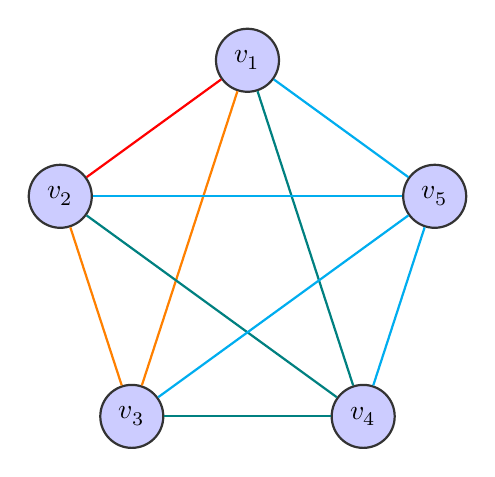
\begin{tikzpicture}[
% Style for the nodes (vertices)
node style/.style={
circle,
draw=black!80,
fill=blue!20,
thick,
minimum size=8mm
}
]

% Place 5 nodes evenly along a circle
\foreach \i in {1,...,5} {
\node[node style] (v\i) at ({90 + (\i-1)*72}:2.5cm) {$v_{\i}$};
}

% STEP 1: Node 1 is placed. (0 connections)

% STEP 2: Node 2 is added. Connects back to Node 1.
\draw[thick, red] (v2) -- (v1);

% STEP 3: Node 3 is added. Connects back to Nodes 1 and 2.
\draw[thick, orange] (v3) -- (v1);
\draw[thick, orange] (v3) -- (v2);

% STEP 4: Node 4 is added. Connects back to Nodes 1, 2, and 3.
\draw[thick, teal] (v4) -- (v1);
\draw[thick, teal] (v4) -- (v2);
\draw[thick, teal] (v4) -- (v3);

% STEP 5: Node 5 is added. Connects back to Nodes 1, 2, 3, and 4.
\draw[thick, cyan] (v5) -- (v1);
\draw[thick, cyan] (v5) -- (v2);
\draw[thick, cyan] (v5) -- (v3);
\draw[thick, cyan] (v5) -- (v4);

\end{tikzpicture}
\caption{Visualising network accumulation: \textcolor{red}{1} + \textcolor{orange}{2} + \textcolor{teal}{3} + \textcolor{cyan}{4} = 10 total connections.}
\label{fig:colored_graph}
\end{figure}

For any graph, one can calculate the number of connections or edges for
\(n\) nodes or vertices using the degree-edge formula. For the complete
graph specifically, one can use this formula or a combinatoric argument
to find that there are \({n \choose 2} = \frac{1}{2}n(n-1)\)
connections. One notices that this formula represents the sum of the
first \(n-1\) natural numbers; we will discuss why this is the case
using a network accumulation argument.

Imagine we have a complete graph with a finite number of \(r-1\) nodes.
If we add a new node, then to create a complete graph of \(r\) nodes, we
need to add \(r-1\) new connections. Consider first the complete graph
with \(r=1\) node: this has \(k = r-1 = 0\) connections. Moving to
\(r=2\) nodes, we must add \(r-1=1\) connection. For \(r=3\) nodes, we
have to add \(r-1=2\) connections to the previous \(1\) connection,
yielding \(k=1+2=3\) connections. Continuing in this manner (which can
be formalized using mathematical induction), we find that the number of
connections for a complete graph with \(n \in \N\) nodes is:

\[k = \sum_{r=1}^{n}(r-1)=1+2+\dots+n-1 = \frac{1}{2}n(n-1)\]

To illustrate this visually, we look at the case of 5 nodes in Figure
\ref{fig:colored_graph}:

\begin{itemize}
\tightlist
\item
  Start with node \(v_1\). When adding \(v_2\), 1 connection is
  established between them (red).
\item
  Add \(v_3\), creating an additional 2 connections from \(v_1\) and
  \(v_2\) to \(v_3\) (orange).
\item
  Add \(v_4\), establishing a further 3 connections from \(v_1\),
  \(v_2\), and \(v_3\) to \(v_4\) (green).
\item
  Finally, add \(v_5\) for the final 4 connections from \(v_1\),
  \(v_2\), \(v_3\), and \(v_4\) to \(v_5\) (blue).
\end{itemize}

\subsection{\texorpdfstring{\(k\) Connections: How Many Nodes
\(n\)?}{k Connections: How Many Nodes n?}}\label{k-connections-how-many-nodes-n}

If the number of connections \(k\) is known, we must solve the formula
derived above for \(n\):

\[\frac{1}{2}n(n-1) = k\]

Using the quadratic formula, the solution for the number of nodes with
\(k\) connections in a complete graph is:

\[n  = \frac{1+\sqrt{1+8k}}{2}\]

As a graph cannot contain a fractional number of nodes, to guarantee at
least \(k\) connections we use the ceiling function
\((\lceil \cdot \rceil)\) to round up to the nearest integer:

\[n  = \left\lceil \frac{1+\sqrt{1+8k}}{2}\right\rceil\]

Let us say we require at least one hundred connections (\(k=100\)). The
number of nodes needed is:

\[n = \left\lceil \frac{1+\sqrt{1+800}}{2}\right\rceil= 15\]

In fact, \(n=15\) corresponds exactly to:

\[k = \frac{1}{2}\cdot 15\cdot14 = 105\]

connections.

\subsection{Asymptotics and Geometry of
Connections}\label{asymptotics-and-geometry-of-connections}

The number of connections \(k\) in a complete graph scales
asymptotically as:

\[k = \frac{1}{2}n(n-1) \sim \frac{1}{2}n^2\]

Asynchronously, the number of connections grows quadratically, meaning
\(k = \mathcal{O}(n^2)\). While this leading-term approximation captures
the dominant behavior, the absolute error grows linearly with \(n\):

\[\left| \frac{1}{2}n(n-1) - \frac{1}{2}n^2 \right| = \frac{1}{2}n\]

Thus, while the absolute error diverges as \(n \to \infty\), the
relative error asymptotically vanishes.

Let us denote a complete graph with \(n\) vertices by the standard
notation \(K_n\). If the complete graph is arranged symmetrically in a
circular fashion, an interesting geometrical pattern emerges (see Figure
\ref{fig:large_complete_graphs}):

\begin{description}[leftmargin=1.8cm, labelwidth=1.6cm, align=left]
    \item[For even $n$:] The edges acting as true diameters (connecting diametrically opposed pairs of vertices) intersect perfectly at the geometric center of the circle, forming a central hub. Moving outward from this center point, the overlapping chords weave together to form an increasing number of concentric, nested inner rings.
    \item[For odd $n$:] No edge can act as a true diameter, meaning all lines bypass the absolute center. This creates a completely clear, circular void at the dead center. As $n$ increases, the radius of this innermost empty circle decreases, while an increasing number of distinct concentric rings form outside of it.
    \item[As $n \rightarrow \infty$:] The discrete vertices converge into a continuous circle, and the $\mathcal{O}(n^2)$ growth of intersecting chords yields an infinitely dense mesh. In the limit, this mesh manifests as a smooth, radially symmetric gradient that is heavily shaded at its core and fades out toward the perimeter.
\end{description}

\begin{figure}[H]
\centering
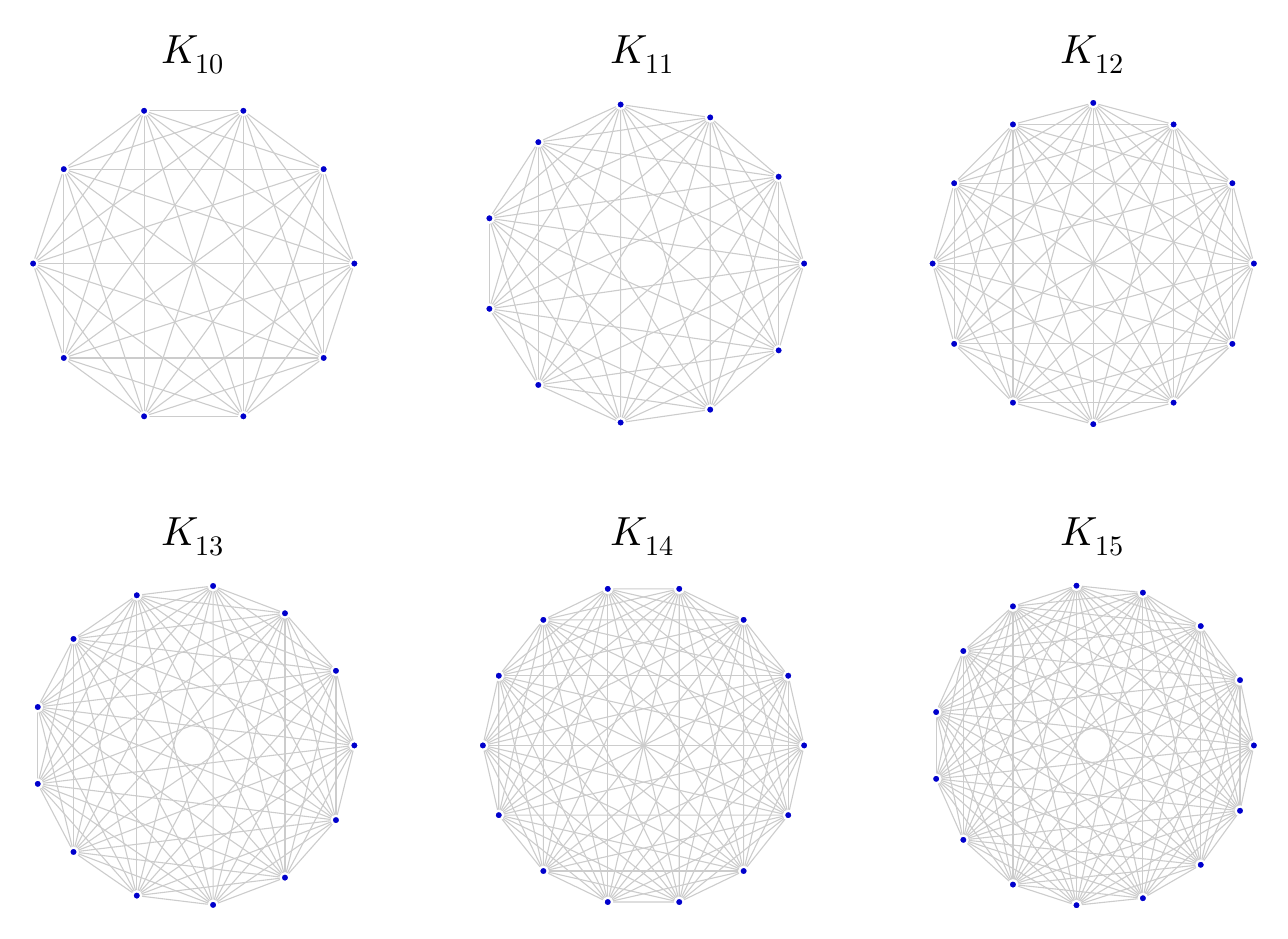
\begin{tikzpicture}[x=1.2cm, y=1.2cm, scale=0.85, every node/.style={transform shape}]
% Loop through the larger graphs from 10 to 15
\foreach \N in {10,...,15} {

% Arrange them in a clean 2-row, 3-column grid
\pgfmathtruncatemacro{\index}{\N-10}
\pgfmathtruncatemacro{\row}{\index/3}
\pgfmathtruncatemacro{\col}{mod(\index,3)}

% Optimized spacing to prevent page clipping
\begin{scope}[shift={(\col*5.6, -\row*6.0)}]

% Heading for each graph
\node[font=\LARGE\bfseries] at (0, 2.6) {$K_{\N}$};

\def\graphradius{2.0}

% Step 1: Draw all internal edges
\foreach \i in {1,...,\N} {
\foreach \j in {\i,...,\N} {
    \ifnum\i=\j\else
    \draw[black!20, thin] ({360/\N * \i}:\graphradius) -- ({360/\N * \j}:\graphradius);
    \fi
}
}

% Step 2: Draw nodes cleanly on top
\foreach \i in {1,...,\N} {
\node[circle, fill=blue!80!black, draw=white, inner sep=1.3pt, thick] 
at ({360/\N * \i}:\graphradius) {};
}

\end{scope}
}
\end{tikzpicture}
\caption{Close-up view of large complete graphs $K_{10}$ through $K_{15}$. Notice the stark visual contrast at the absolute center between the even graphs ($K_{10}, K_{12}, K_{14}$) which possess a sharp central intersection point, and the odd graphs ($K_{11}, K_{13}, K_{15}$) which maintain a completely clear, circular void in the middle.}
\label{fig:large_complete_graphs}
\end{figure}

\subsection{An Interesting Example of a Complete Graph: the
Universe!}\label{an-interesting-example-of-a-complete-graph-the-universe}

Though I am not a physicist, exploring the nature of cosmic forces leads
to a fascinating realization: because every particle interacts with
every other particle across spacetime, the universe is, at its most
fundamental level, the ultimate manifestation of a complete graph.




\end{document}
